% latexmk -xelatex file.tex

\documentclass[12pt, aspectratio=169]{beamer}
\linespread{1.15}
\newcommand{\university}{Санкт-Петербургский политехнический университет Петра Великого}
\newcommand{\faculty}{}
\newcommand{\department}{}

\newcommand{\city}{Санкт-Петербург}
\newcommand{\num}{ № 1}
\newcommand{\docname}{Разработка цифровой модели РТК "Ровер" и отладка САУ в цифровой среде }
\newcommand{\tutorname}{П. А. Гаврилов}
\newcommand{\studentname}{Г. В. Казанцев}
\newcommand{\group}{3331506/00401}
\usepackage{setspace}
\usepackage{fontspec}
\usepackage{xunicode}
\usepackage{xltxtra}
\usepackage{dsfont}
\usepackage{multicol}
\usepackage{array}
\usepackage{xecyr}
\usepackage{hyperref}
\usepackage{polyglossia}
\usepackage{graphicx}
\usepackage{listings}
\usepackage{media9}
\usepackage{capt-of}
\usepackage[darktherm, useprogressbar, classmode=all]{ubersbeamer1}
\usepackage[figurename=Рис.]{caption}


\begin{document}
    \AtBeginSection[] 
    {
      \begin{frame}{Содержание}
        \tableofcontents[currentsection,hideallsubsections]
      \end{frame}
    }

    \AtBeginSubsection[]
    {
      \begin{frame}{подсекции}
        \tableofcontents[currentsubsection, hideothersubsections, sectionstyle=show/hide, subsectionstyle=show/shaded/hide]
      \end{frame}
    }

    %%%%%%%%%%%%%%%%%%%%%%%%%%%%%%%              Главный слайд             %%%%%%%%%%%%%%%%%%%%%%%%%%%%%%%%%%%%%%%%
    \title[\docname]{\docname}
    %\subtitle{для кого может быть сделана это?}
    \author[\tutorname]{\small Выполнил: ст. гр. \group \ \studentname\\[1mm]{\small Руководитель: \tutorname\\[-30mm]}}
    \date[\date]{\the\year\\[17mm]{ \city\\[-25mm]}}
    \frame{\titlepage}
    %\institute[\university]{\university \\ \faculty}

    %%%%%%%%%%%%%%%%%%%%%%%%%%%%%%%              Обоснование темы НИР              %%%%%%%%%%%%%%%%%%%%%%%%%%%%%%%%%%%%%%%%
    \begin{frame}{Обоснование темы НИР}\relax
      \vspace{-1.5cm}
      \begin{flushleft}
        \begin{itemize}
          \item Технологии цифровых моделей позволяют создать виртуальную математическую модель реальной физической системы.
          \item С помощью симуляций можно воссоздать поведение робота в текущей конфигурации до его физической реализации, что 
        позволит заранее исследовать систему в различных условиях. 
        \end{itemize}
      \end{flushleft}
    \end{frame}

    \section{Проделанная работа}

    %%%%%%%%%%%%%%%%%%%%%%%%%%%%%%%              Цели и задачи              %%%%%%%%%%%%%%%%%%%%%%%%%%%%%%%%%%%%%%%%
    \begin{frame}{Цели и задачи}
      \highgreen{\texttt{\string Целью работы}}  является создание САУ для РТК <<Ровер>> в MSC Adams View в совместной симуляцией с Matlab.
      \\ Задачи:
      \begin{itemize}
        \item \small обзор альтернативых решений;
        \item \small изучение программы Adams View и ее плагина Adams Control;
        \item \small подготовка модели РТК <<Ровер>> для симуляций в Adams View \& Matlab;
        \item \small проверочный расчет объемов и моментов инерции для каждого жлемента конструкции;
        \item \small создание САУ для сравнение кинематики цифровой модели и реального робота;
        \item \small подготовка ячеек полигона для симуляций в Adams View \& Matlab;
        \item \small итговая отладка работы цифровой модели.
      \end{itemize}
    \end{frame}

    %%%%%%%%%%%%%%%%%%%%%%%%%%%%%%%              Matlab Simulink              %%%%%%%%%%%%%%%%%%%%%%%%%%%%%%%%%%%%%%%%
      \begin{frame}{Adams View <-> Adams Control <-> Matlab <-> Simulink}
        \begin{columns}[T,onlytextwidth]
                \begin{column}{0.65\textwidth}
                  \vspace{-0.5cm}
                        \begin{itemize}
                                \item \small Стандарт FMI (Functional Mock-up Interface)-
                                интерфейс для переноса и совместного использования моделей в различных средах моделирования.
                                \item \small Во время симуляции происходит постоянный обмен данными.
                                \item \small MSC Adams (автоматический динамический анализ механических систем) представляет собой программную систему
                                 для моделирования динамики нескольких тел.
                                 Решатель программного обеспечения для моделирования работает в основном на C++.  
                        \end{itemize}
                \end{column}
                \begin{column}{0.35\textwidth}
                \vspace{0.5cm}
                  \center{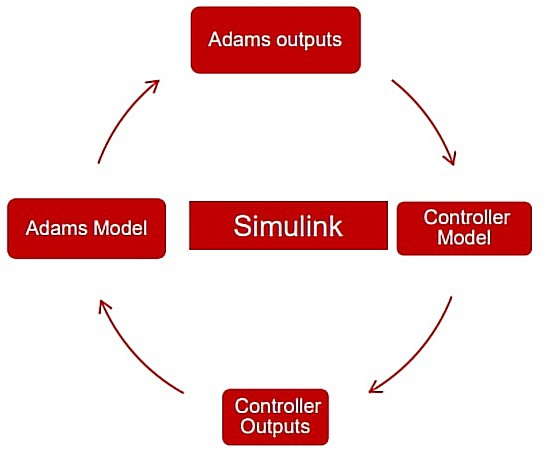
\includegraphics[width=5.0cm]{src/images/adams_simulink_scheme.jpg} \\ \footnotesize Рис. 1 - Ко-симуляция}
                \end{column}
        \end{columns}
      \end{frame}

%\highgreen{\texttt{\string\highgreen\{text\}}}
  

    %%%%%%%%%%%%%%%%%%%%%%%%%%%%%%%              Что сделано              %%%%%%%%%%%%%%%%%%%%%%%%%%%%%%%%%%%%%%%%
    \begin{frame}{Импорт модели из SolidWorks в Adams. Модель схвата}\relax
          \begin{columns}[T,onlytextwidth]
            \begin{column}{0.5\textwidth}
              \vspace{-0.5cm}
              \center{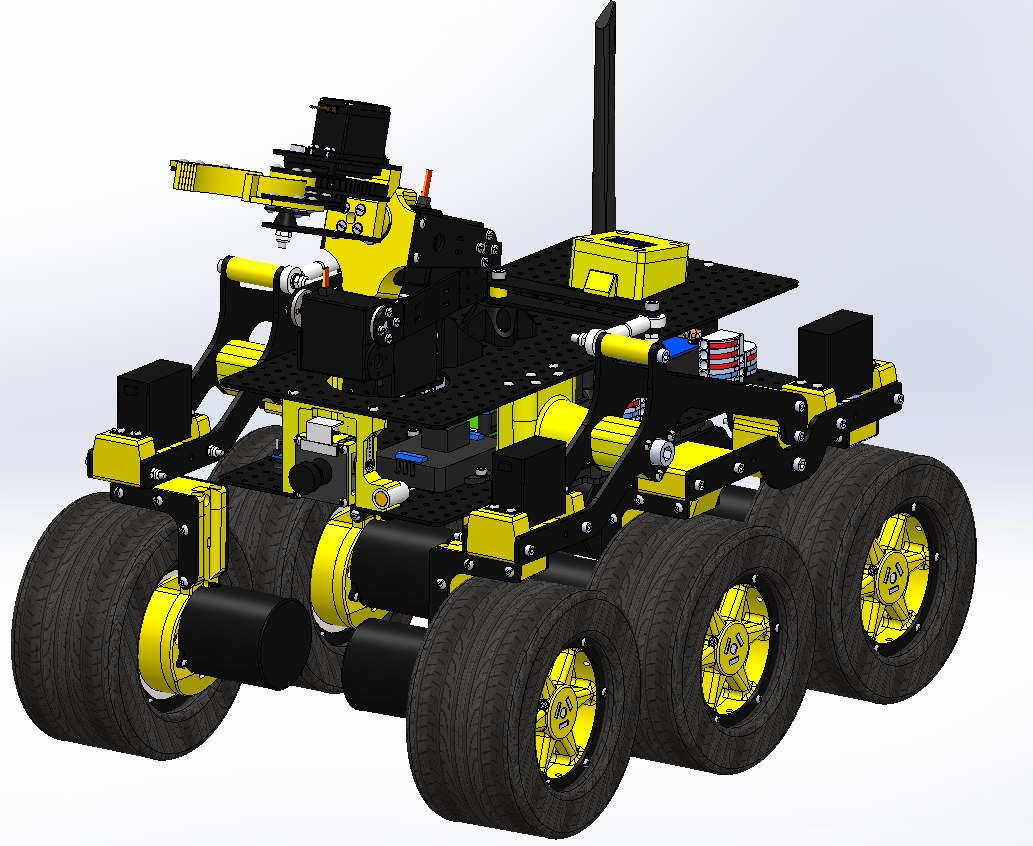
\includegraphics[width=6.5cm]{src/images/Rover.png} \\ \footnotesize Рис. 2 - РТК <<Ровер>>}
            \end{column}
            \begin{column}{0.5\textwidth}
            \vspace{-1.0cm}
              \center{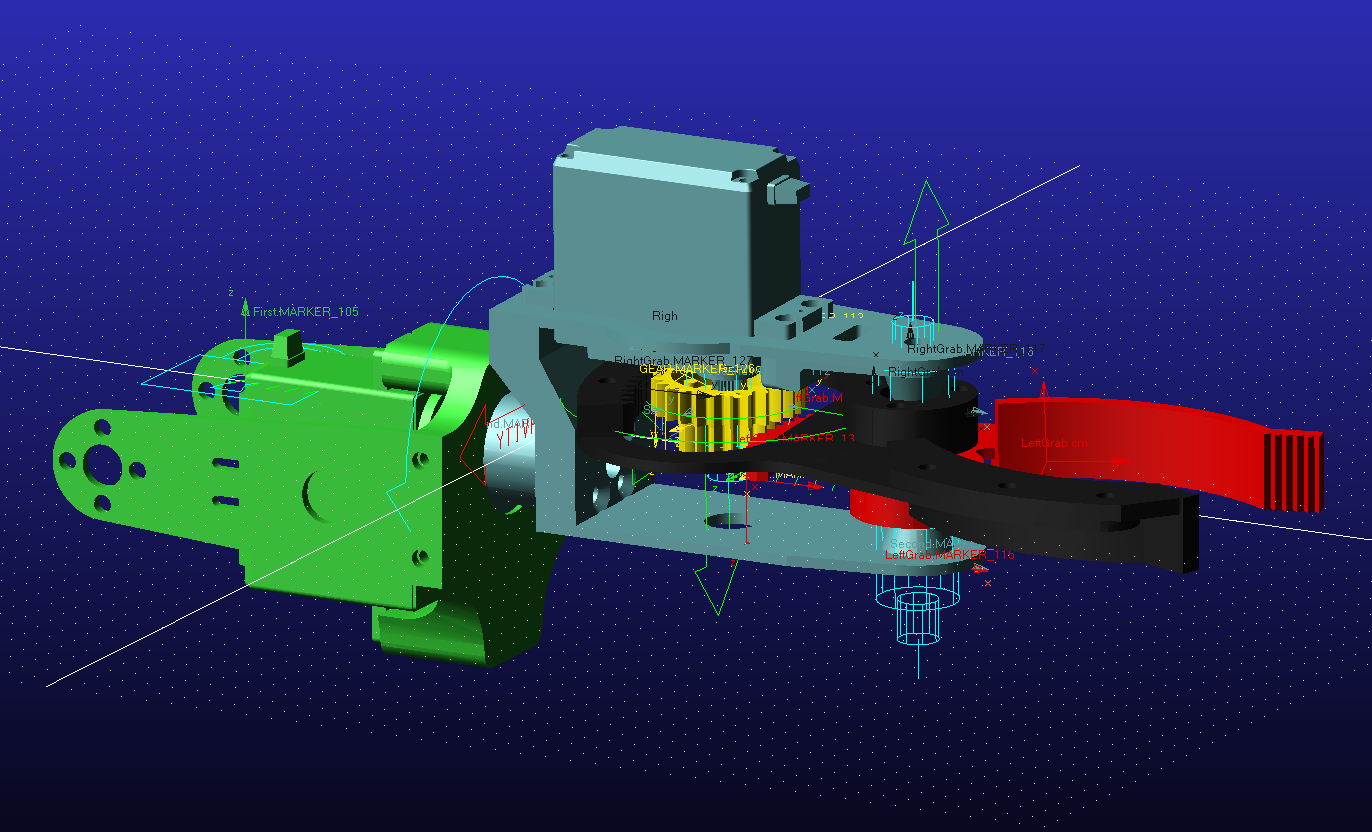
\includegraphics[width=6.5cm]{src/images/rover_sxvat.png} \\ \footnotesize Рис. 3 - Схват РТК <<Ровер>>}
               \\\begin{flushleft} Модель схвата импортирована из SolidWorks с правильной геометрией.\end{flushleft}
            \end{column}
    \end{columns}
    \end{frame}
    %%%%%%%%%%%%%%%%%%%%%%%%%%%%%%%              Обратная связь             %%%%%%%%%%%%%%%%%%%%%%%%%%%%%%%%%%%%%%%%
    \begin{frame}{Импорт модели из SolidWorks в Adams. Модель схвата}\relax
      \begin{columns}[T,onlytextwidth]
        \begin{column}{0.5\textwidth}
          \vspace{-0.5cm}
          \center{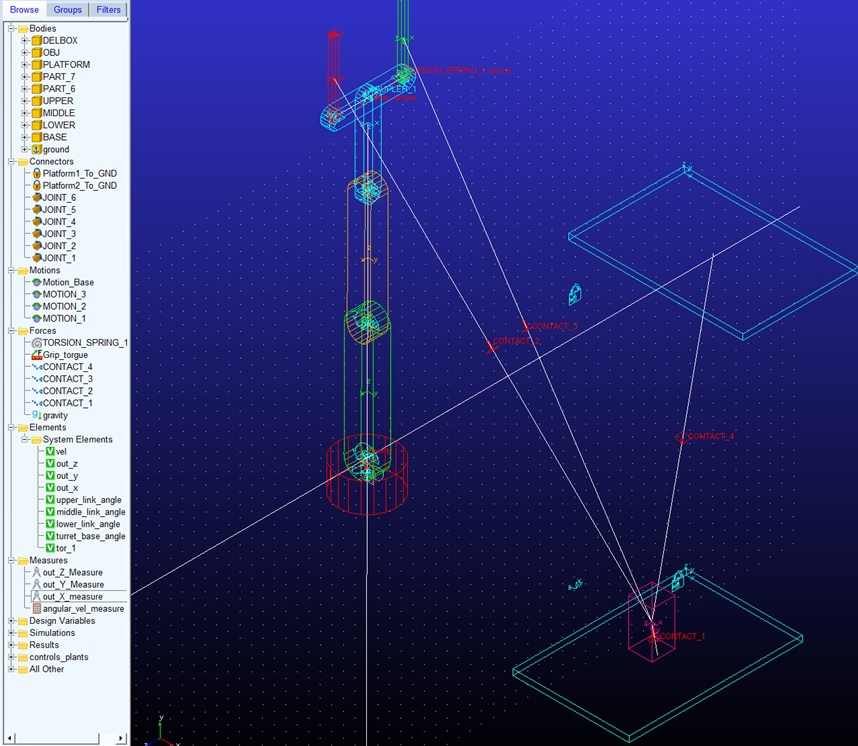
\includegraphics[width=6.5cm]{src/images/backward_link2.jpg} \\ \footnotesize Рис. 4 - Интерфейс Adams View}
        \end{column}
        \begin{column}{0.5\textwidth}
          \vspace{-0.0cm}
          \center{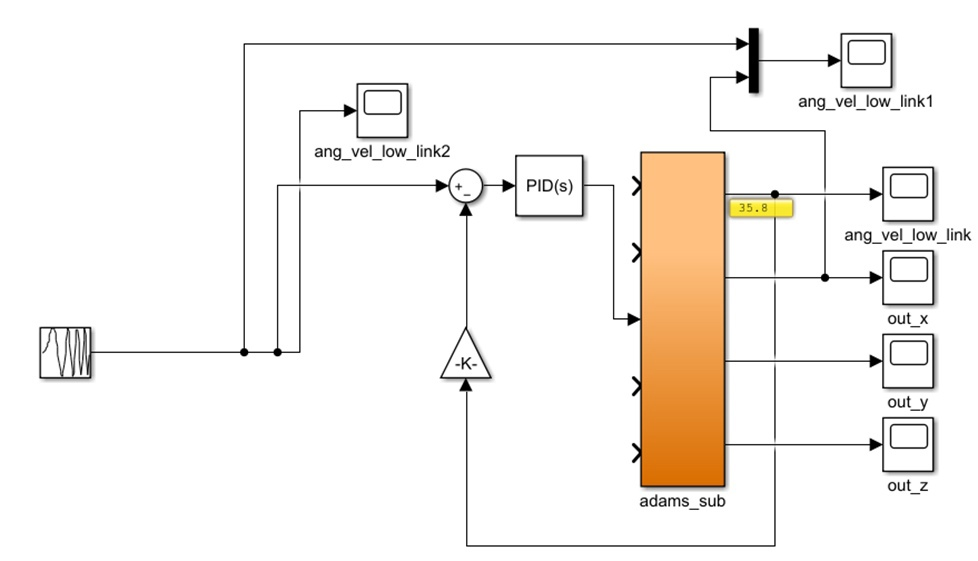
\includegraphics[width=6.5cm]{src/images/backward_link1.jpg} \\ \footnotesize Рис. 5 - Обратная связь в Matlab \& Simulink}
        \end{column}
    \end{columns}
    \end{frame}


    %%%%%%%%%%%%%%%%%%%%%%%%%%%%%%%              Сроки              %%%%%%%%%%%%%%%%%%%%%%%%%%%%%%%%%%%%%%%%
    \section{Сроки}
    \begin{frame}{Сроки выполнения}\relax
      \vspace{-1.5cm}
      \begin{flushright}
        Таб. 1 - План работ
      \end{flushright}
      \vspace{-0.5cm}
      \resizebox {15cm}{!}
      {
      \begin{tabular}{c l c}
        \hline 
        № & Описание задачи 1 & Срок выполнения \\
         \hline
          1 & Обзор альтернативых решений & 01.09.2023-20.09.2023 \\ \hline
          2 & Теоритическая и практическая работа с MSC Adams View & 01.09.2023-30.10.2023 \\ \hline
          3 & Подготовка модели РТК <<Ровер>> для исследования & 20.10.2023-10.11.2023 \\ \hline
          4 & Кинематическое и динамическое исследование модели & 10.11.2023-01.12.2023 \\ \hline
          5 & Численное сравнение одометрии модели и реального робота & 20.12.2023-20.01.2024 \\ \hline
          6 & Импорт испытательного полигона (не менее двух ячеек) & 20.01.2024-20.03.2024 \\ \hline
          7 & Итоговая проверка и отладка работы цифровой модели & 20.03.2023-20.04.2024 \\ \hline
        \end{tabular}
      }
        \cscfootnote{\small *Новые задачи могут добавляться по ходу работ.}
    \end{frame}


    \section{Список литературы}
%%%%%%%%%%%%%%%%%%%%%%%%%%%%%%%              Список литературы            %%%%%%%%%%%%%%%%%%%%%%%%%%%%%%%%%%%%%%%%
    \forcewidefootnote=-1
    \begin{frame}[allowframebreaks]
      \frametitle{Список литературы}
      \vspace{-1.0cm}
      \bibliographystyle{plain}
        \begin {thebibliography}{9}
        \bibitem{textbook} \footnotesize Гайдук, А.Р. Теория автоматического управления в примерах и задачах с решениями в MATLAB: 
        Учебное пособие. 3-е изд., стер / А.Р. Гайдук, В.Е. Беляев и др. — СПб.: Лань, 2016. — 464 c.
        \bibitem{textbook} \footnotesize İlgen S., Durdu A., Gülbahçe E., Çakan A., Sliding Mode Control of a Two-link Robot
        Manipulator Using Adams and Matlab Software // 2018 6th International Conference on Control Engineering \& Information Technology (CEIT) 
        (25-27 October 2018, Istanbul, Turkey) - , Istanbul, 2018.
        \bibitem{textbook} \footnotesize Parthasarathy T., Srinivasaragavan V., Santhanakrishnan S., ADAMS-MATLAB Co-Simulation of A Serial Manipulator 
        // MATEC Web of Conferences 95, (6-7 november, 2017).
      \end{thebibliography} 
    \end{frame}
    \forcewidefootnote=0
\end{document}